\chapter{Testbench vs Selenium}
\label{ch:testbenchvsselenium}
In this chapter we will summarize advantages of using TestBench against
Selenium.

\section{API built specifically for Vaadin components}
Selenium operates on the DOM of the Web page and provides basic methods of
Web elements like ``click'' or ``sendKeys''. For example, to find a value in the Vaadin table
 when using Selenium, a developer needs to understand how the Vaadin component
 is built and prepare a selector to find a specific row and cell in it, which is often error prone even
 for advanced front-end developers.
 
TestBench provides an alternative selector variant with a greater abstraction for Vaadin components.
This makes it easier and faster to write tests and also protects test scripts
from potential changes made to the client side implementation of Vaadin components.
 Using the previous example to get a row or cell of the Table by index you need two lines of code
 see~\ref{lst:testbench1}.
    \lstset{style=a1listing}
    \begin{lstlisting}[caption=Get Vaadin Table cell Value,label={lst:testbench1}]
TableElement table = getTableElement();
String value = table.getRow(0).getCell(1).getValue();
  \end{lstlisting}

Testbench is backward compatible with Selenium and if a developer ends up in a
situation where Testbench lacks helper methods, he can write the test or a helper method with plain Selenium.

In Selenium tests, elements are picked from the page by identifiers.
Adding identifiers to all elements complicates the source code. When using Testbench you can
search elements by class or caption, which makes navigating on the page easier.
	
\section{Client server communication}
As mentioned in section~\ref{ch:reasontestbenchdevelopment}
Selenium does not handle client server communications in Vaadin
application. TestBench fixes this problem.

Before calling any client side code, for example, setting a value of a
text field, TestBench waits for server side code to finish. When event happens
on the client side, TestBench sets a boolean value ``hasRequestToServer'' to
true and sends a request to the server side. When the server side finishes its
work, it returns a response and the client side sets the ``hasRequestToServer''
flag back to false. While there is a request to a server executing all TestBench
methods on the client are suspended see figure \ref{fig:clientServerTestbench}.  
	\begin{figure}
	\centering
	
\includegraphics[width=0.75\textwidth]{clientServerTestbench}
	\caption{Client server synchronization in TestBench}
	\label{fig:clientServerTestbench}
	\end{figure}

\section{Screenshot comparison}
\label{sec:screencompare}
Since version 4.0.0 TestBench has an API for comparing screenshots. This 
feature was introduced to help users to test UI of the application. We believe
that User Experience (UX) is very important in Web applications, and an
important part of UX is look and feel of the application.

In Web applications styling is done with CSS or SCSS. The downside of CSS 
is that changing CSS rule for one selector may affect many elements on the
web page. For example change the width or margin of one element may ruin an
appearance of the whole Web page.

Manual UI testing is very difficult, because of the two main challenges:
\begin{enumerate}
  \item After some time the tester looses his concentration and does not see
  errors
  \item Small details in applications with rich UI is hard to notice for a
  human. In other words if you have several text fields and buttons in different
  tabs or windows in the application it is hard to notice that some of them are
  not aligned.
\end{enumerate}

Both these two problems can be solved with automatic screenshot comparison.
ImageComparesment class has an overloaded compare method which takes either an
image or a path to the reference screenshot. The comparison is done in 16x16
blocks comparing RGB values of the every pixel in this block. If there are
differences in images these parts are marked with color, so it is easier for a
tester to find out what was the problem with the test see
\ref{fig:failedscreen} and \ref{fig:failedscreenmarked}.

	\begin{figure}
	\centering
	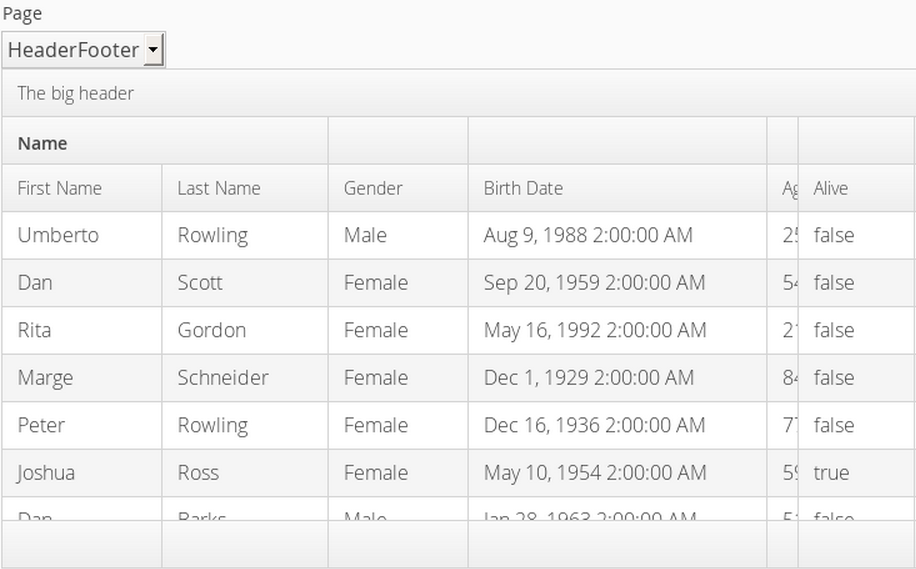
\includegraphics[width=0.75\textwidth]{screen_fail}
	\caption{Reference screenshot}
	\label{fig:failedscreen}
	\end{figure}

	\begin{figure}
	\centering
	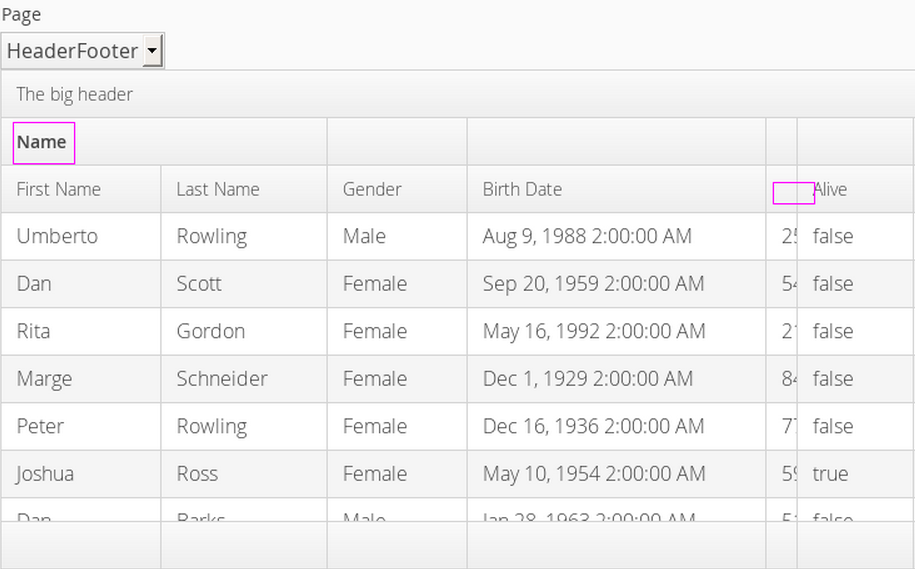
\includegraphics[width=0.75\textwidth]{screen_fail_marked_error}
	\caption{Screenshot with emphasized error}
	\label{fig:failedscreenmarked}
	\end{figure}

TestBench test can also be configured to automatically take screenshots of the failing tests by adding
a ``screenshot on failure rule'' see \ref{lst:screenshotOnFailue}. Automatically
taking screenshots of failing tests helps developers to narrow the
scope of a potential problem much faster.

\lstset{style=a1listing}
  	\begin{lstlisting}[caption=Adding screenshot on failure	rule,label={lst:screenshotOnFailue}]
@Rule
public ScreenshotOnFailureRule screenshotOnFailureRule =
	 new ScreenshotOnFailureRule(this, true);
	\end{lstlisting}

\section{Parallel testing}
\label{sec:paralelTesting}
As mentioned in section~\ref{ch:selenium} Selenium Grid allows to run
tests on different machines with different configuration. Unfortunately
Selenium does not provide a ready made solution to start those tests in
parallel, the developer can  use a maven surefire plugin \cite{sureFireExample} 
or JUnit ``ParallelComputer" class \cite{junitParallelComputer}. This requires
additional work for example to use ten parallel threads for running tests using
surefire plugin you need to add this XML snippet \ref{lst:surefirePom}
to your POM file.

\lstset{style=console}
\begin{lstlisting}[caption=Get Vaadin Table cell Value,label={lst:surefirePom}]
<plugins>
    [...]
      <plugin>
        <groupId>org.apache.maven.plugins</groupId>
        <artifactId>maven-surefire-plugin</artifactId>
        <version>2.19</version>
        <configuration>
          <parallel>methods</parallel>
          <threadCount>10</threadCount>
        </configuration>
      </plugin>
    [...]
</plugins>
\end{lstlisting}	

TestBench4 introduced a ``ParallelTest'' class which thread pool and execute tests
in separate threads in parallel. The amount of threads can be changed by
calling ``Parameters.setMaxThreads() method. Besides listing~\ref{lst:starthub2}
shows that a developer needs to use different WebDrivers for running his test in
different Web browsers or for running on Selenium Hub. TestBench uses Java
annotations ``@RunLocally'' \ref{lst:testBenchLocally} and ``RunOnHub''
\ref{lst:testBenchRunOnHub}.
``RunOnHub'' annotation sets remote Web Driver capabilities for Chrome, Firefox and Internet Explrorer 9,
10,11 by default. We believe that these adjustments in ``ParallelTest'' class
minimize the amount of extra code and developers effort needed to setup a test
environment.
\lstset{style=a1listing}
\begin{lstlisting}[caption=Run test in local Chrome browser locally,label={lst:testBenchLocally}] 
@RunLocally(Browser.CHROME)
public class LocalTest extends ParallelTest { 
	@Test
	public void test1() {
		getDriver().get("http://demo.vaadin.com/dashboard/");
	}
}
\end{lstlisting}

\lstset{style=a1listing}
\begin{lstlisting}[caption=Run tests on Selenium hub on http://192.168.1.2, label={lst:testBenchRunOnHub}]
@RunOnHub(http://192.168.1.2)
public class LocalTest extends ParallelTest {
@Test
public void test1() {
	getDriver().get("http://demo.vaadin.com/dashboard/"); }
}
\end{lstlisting}

